%!TEX root = Report.tex



\section{Introduction}

\subsection{Motivation}
Due to a recent legislative regulation of noise in work environments, active noise cancellation in motorcycle helmets has gained increased attention in the last years. With the goal of preventing noise induced hearing loss (NIHL), a recent European  court order has set the maximum noise level for a worker to tolerate during a regular working day to 87 dB. These regulations are very difficult to fulfill with existing technologies. Moreover, occupational motorcyclists of all kinds are specially at high risk of NIHL. This is why the search for possible technical innovations to enhance noise cancellation has become a pressing issue in the face of these recent developments. 

\subsection{Objectives}

The approach stated in \ref{} proposes the combination of a feed-forward controller with a feedback controller for satisfactory noise-canceling results, with the special consideration of the critical frequency band between 20 Hz and 1.5 kHz where the highest sound pressure levels are perceived. This study has the objective of modeling the acoustic systems for both controllers, and subsequently performing system identification on them using externally gathered data.

\subsection{Organization}

In section \ref{}, I will describe the detailed acquisition and characteristics of the measured data obtained for this study. After having introduced the experimental parameters, I will show and explain the block diagrams in section \ref{} describing the system models for the acoustic feed-forward and feedback setups. Section \ref{} will explain the details to the system identification techniques chosen for this study and their results using the external data. In the last sections I will discuss the results and show my conclusions.


\section{Setup}
The data acquisition was done by Prof. S\'{a}nchez Pe\~{n}a, who requested a system description of the acoustic setups. During the experiments, three different people and two different setups - one for the feedback controller and one for the feed-forward controller -  were used. For the feed-forward setup, the first microphone was placed on the chin of the user and the second one in the ear canal, both inside the helmet (Figure \ref{}). An external speaker, placed in front of the user, was then used to produce the sound to be measured. Both signals of the microphones were saved in the channels of a stereo audio file without compression (44.1 kHz/16 bit).\\

\begin{figure}[H]
\centering
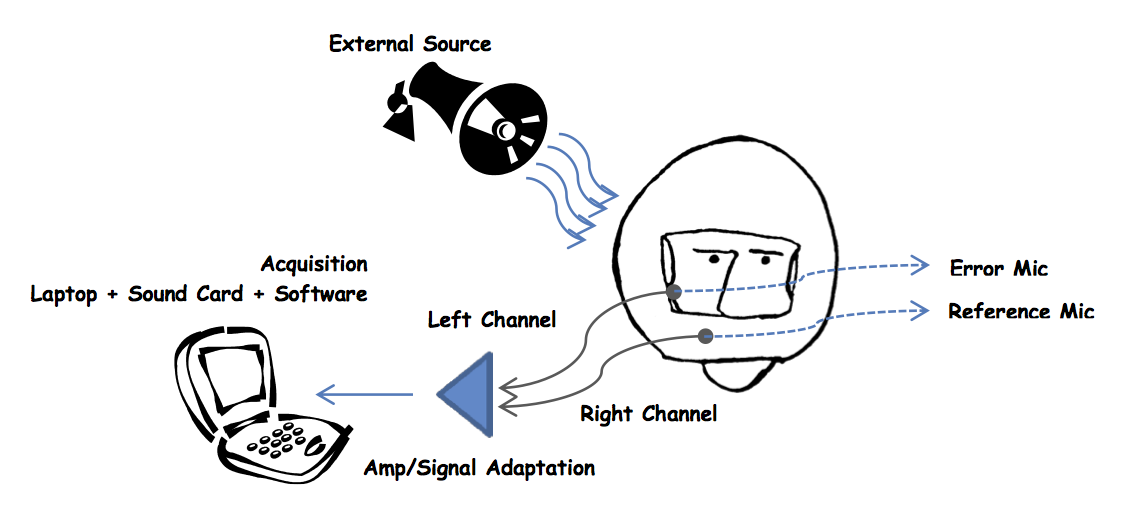
\includegraphics[width=1.0\textwidth]{pics/setupff}
\caption{}
\label{pic:}
\end{figure}

For the feedback setup, only one microphone was placed in the ear canal (inside the helmet). The sound was then generated by a headphone outside the helmet at ear level (Figure \ref{}). The measured headphone voltage was the second recorded signal, which was also saved in a stereo audio file together with the ear microphone signal.

\begin{figure}[H]
\centering
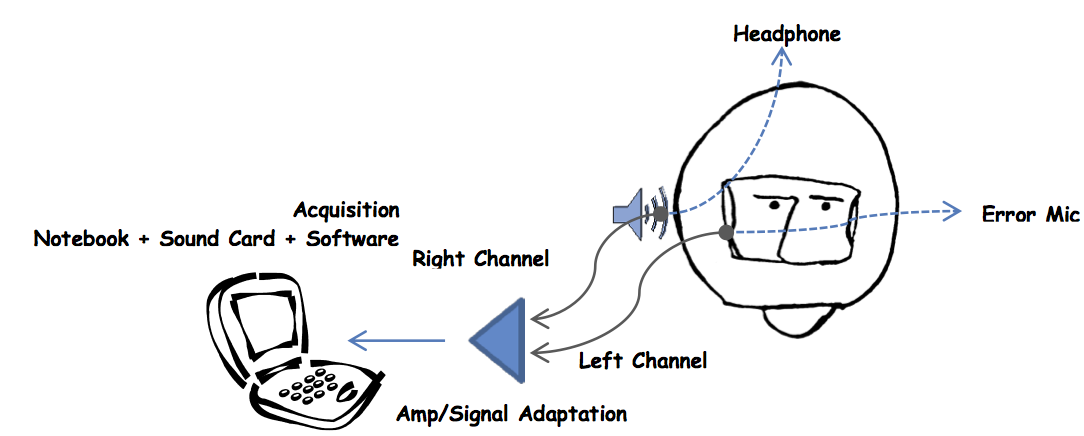
\includegraphics[width=1.0\textwidth]{pics/setupfb}
\caption{}
\label{pic:}
\end{figure}

\section{Input Signals}

During the experiments, the speaker and headphone generated two types of signals for the measurements: A sinusoidal sweep, which gradually increases from 20 Hz to 4 kHz, and white noise run through a low pass filter with a cutoff frequency at 5 kHz. The sweep signal experiment was performed twice for each controller setup and both setups where repeated for the three different users. However, only one of the users delivered results of the desired quality. The two other users reported an uncomfortable fit, and the microphone's unintentional rubbing against the skin corrupted the signal. Therefore, I worked with only six pairs of measurements for the identification: Two sweep signals and one filtered noise signal, once for each controller setup.

\begin{figure}[H]
\centering
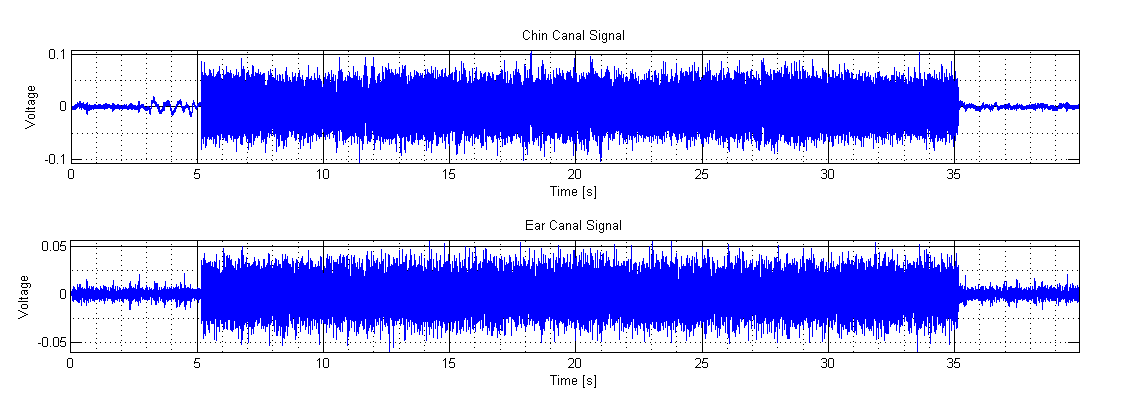
\includegraphics[width=1.0\textwidth]{pics/Noise}
\caption{}
\label{pic:}
\end{figure}

\begin{figure}[H]
\centering
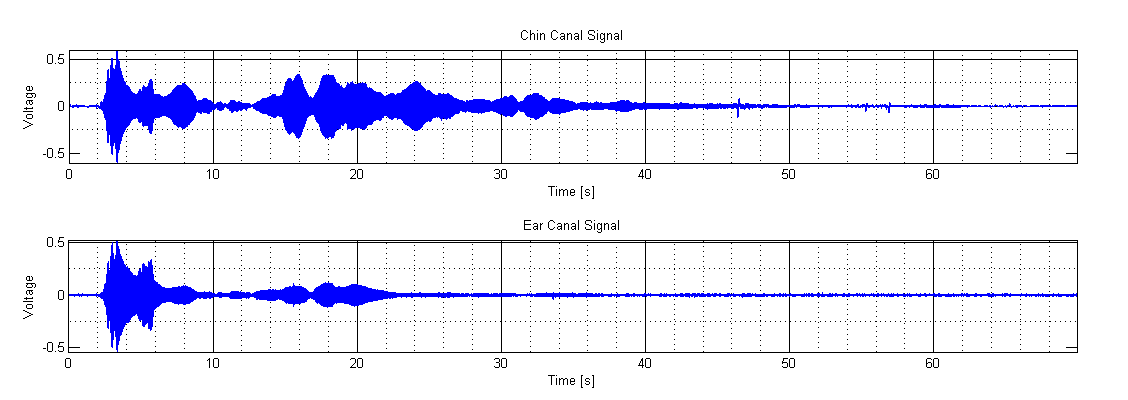
\includegraphics[width=1.0\textwidth]{pics/Sweep}
\caption{}
\label{pic:}
\end{figure}

\section{Modelling}

In the feedback and feed-forward setups we are faced with an input-output behavior. We are interested in seeing how the sound pressure varies between the chin and the direct entry of the ear canal for the feed-forward setup, while the feeback setup examines the sound pressure behavior between the headphone and the ear canal. In the feed-forward setup, the sound wave at the chin would be the input signal, and the sound wave at the ear would be the output. In the case of the feedback setup, the sound wave created by the headphone would be the input and the sound wave at ear level the ouptut. The microphone measurements are corrupted by noise (which we assume to be white noise). Therefore, it is necessary to consider this assumption while choosing a suited model.\\

\begin{figure}[H]
\centering
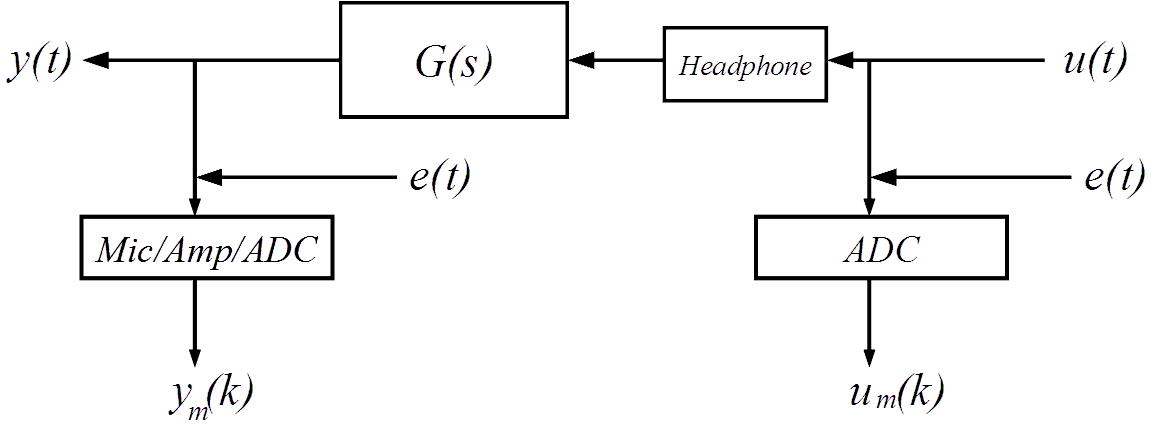
\includegraphics[width=1.0\textwidth]{pics/modelfb}
\caption{}
\label{pic:}
\end{figure}

Figure \ref{} shows the block diagram for the feedback model. The signal chain starts with the analog voltage signal fed to the headphone, which is corrupted by noise. The signal is then transferred into the computer as discrete data with an analog-to-digital converter (ADC) and a preamplifier (\ref{}). Inside the helmet, the sound wave is measured by a microphone, which adds noise, and then converted to discrete data with an ADC and preamplifier.  \\

\begin{figure}[H]
\centering
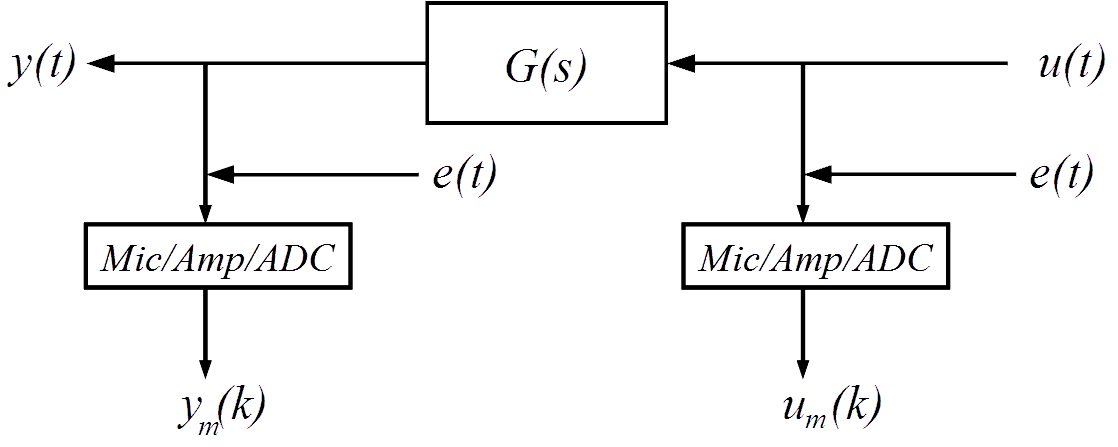
\includegraphics[width=1.0\textwidth]{pics/modelff}
\caption{}
\label{pic:}
\end{figure}

Figure \ref{} illustrates the block diagram for the feed-forward model. The output data is the same as in the other model, but the input is different. The input of the signal chain is the analog sound wave coming from the speaker. The measured input data is given by the chin microphone - again adding noise - and is also converted to to a discrete signal by a ADC and preamplifier.\\

The purpose of this analysis is to determine a model that describes the real acoustic system for control purposes. Using a continuous model as the one shown above makes little sense in the context that a suited controller should be discrete, and thus would require a discrete system. The most logical approach is therefore the inclusion of the electronic setup in the system to be identified, since the use of a controller would anyways require a digital voltage signal as input-output data. The identification model that will be used in this study is the one shown in Figure \ref{}. Here, the transfer function will be discrete, as well as its input and output, for both FF and FB cases. The inputs and outputs are corrupted by discrete white noise.

  \begin{figure}[H]
\centering
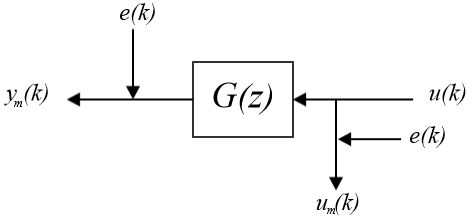
\includegraphics[width=1.0\textwidth]{pics/discrete_model}
\caption{}
\label{pic:}
\end{figure}



\section{Analysis}

In this section I will explain the mathematical methods used for the analysis of the data, with the purpose of finding the transfer functions that describe both systems. Basically, there are three main steps I took to find the transfer functions: Averaging, calculating a non-parametric transfer function, and subspace identification using the N4SID-Algorithm.\\

For the identification process mentioned above, I used the filtered white noise data, since we can average it and it contains information over a higher frequency range. To validate the identification, I used the sweep sign signals.

\subsection{Averaging}

Since white noise is an independent stochastic process (data points are uncorrelated), we can divide the whole measurement into independent data sequences. Averaging is an unbiased operation, helping to reduce the effect of noise. Therefore, we want to maximize the amount of times we subdivide the measurement. However, we don't want to lose resolution in the frequency steps, when doing a discrete Fourier transform.\\

The minimal frequency step we need equals the smallest relevant frequency, which is 20 Hz in our case. We then describe the frequencies in an N-point Fourier transform, using Herz (Hz) as a unit.

\[ f_\text{min} =\left. \omega_k\right|_{k = 1}\frac{f_\text{S}}{2\pi} = \left. \frac{2\pi k}{N}\right|_{k = 1}\frac{f_\text{S}}{2\pi} = \frac{f_\text{S}}{N} \]

Now we can derive the needed amount of data points $N$ per subdivision to preserve the desired frequency resolution.

\[\Rightarrow N = \frac{f_\text{S}}{f_\text{min}} = \frac{44100 \text{ Hz}}{20 \text{ Hz}} = 2205\]
 
Subsequently, we can divide the noise signals of both FF and FB setups into $N_s$ subdivisions of $N = 2205$ data points. A discrete Fourier transform will be used on every subdivision:

\[U_i(e^{j\frac{2\pi n}{N}}) = \frac{1}{N}\sum\limits_{k = 1}^{N }u_i(k)e^{-j\frac{2\pi n}{N}} \quad, \quad Y_i(e^{j\frac{2\pi n}{N}}) = \frac{1}{N}\sum\limits_{k = 1}^{N }y_i(k)e^{-j\frac{2\pi n}{N}}\]

for all $i = 1, ..., N_s$. Here is $u_i(k)$ the $i$th subdivision of the input signal, i.e. the chin signal in the FF model and headphone signal in the feedback model. Similarly $y_i(k)$ is the $i$th subdivision of the output signal, i.e. the ear signal for both models. \\

Now, we can average each Fourier transformed signal:
\[U_\text{av}(e^{j\frac{2\pi n}{N}}) = \frac{1}{N_s}\sum\limits_{k = 1}^{N_s }U_i(k) \quad, \quad Y_\text{av}(e^{j\frac{2\pi n}{N}}) = \frac{1}{N_s}\sum\limits_{k = 1}^{N_s} Y_i(k)\]

Figure \ref{} shows the Fourier transform of the averaged and the non-averaged, complete, noise signal in the headphone channel and in the ear channel. We see a clear reduction of noise in the averaged one.

\begin{figure}[H]
\centering
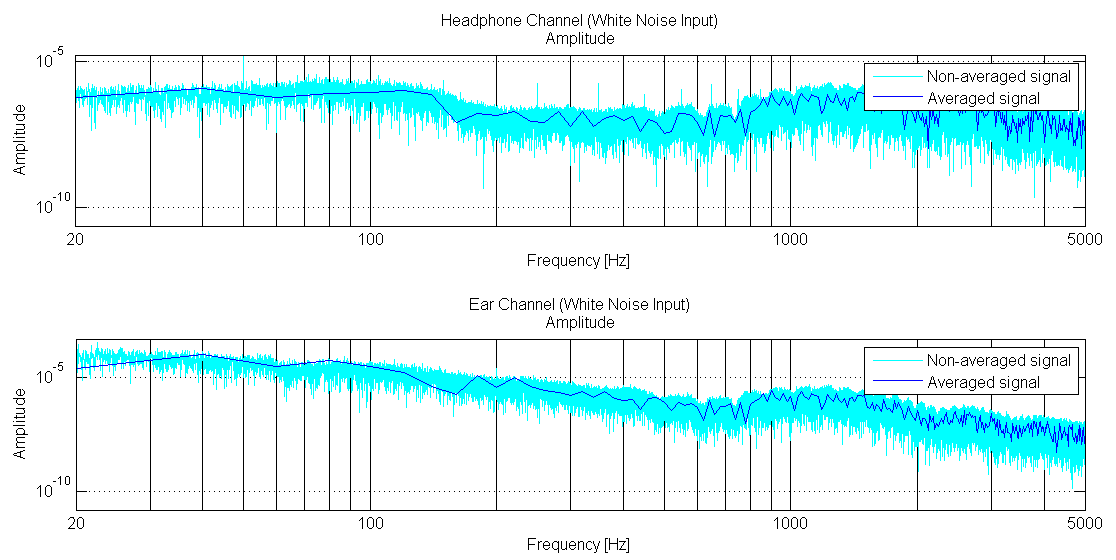
\includegraphics[width=1.0\textwidth]{pics/averagedvsnonaveraged}
\caption{}
\label{pic:}
\end{figure}


\subsection{Empirical Transfer Function}
After this, we can calculate the data points of the non-smoothed empirical transfer function $G_E(e^{j\frac{2\pi n}{N}})$ at the frequencies where the Fourier transformed signals are defined:

\[G_E(e^{j\frac{2\pi n}{N}}) = \frac{Y_\text{av}(e^{j\frac{2\pi n}{N}})}{U_\text{av}(e^{j\frac{2\pi n}{N}})}\]


The empirical transfer function shows a noisy behavior, since our signals are corrupted with noise (it would otherwise show the actual data points of the transfer function). Since the algorithm we will use later to find the parametric description of the system (N4SID Algorithm) works best with data points of a smoothed estimate, we will smooth our empirical transfer function estimate.\\

First we will calculate the autocorrelation of $u(k)$ and cross-correlation of $u(k)$ and $y(k)$:

\[R_{yu}(k) = \frac{1}{N}\sum\limits_{l = 1}^N y(l)u(l-k) \quad , \quad R_{u}(k) = \frac{1}{N}\sum\limits_{l = 1}^N u(l)u(l-k)\]

It can be proved, that the empirical transfer satisfies the following relation: 

 \[G_E(e^{j\frac{2\pi n}{N}}) = \frac{\Phi_{yu}(e^{j\frac{2\pi n}{N}})}{\Phi_{u}(e^{j\frac{2\pi n}{N}})}\]

Where $\Phi_{yu}(e^{j\frac{2\pi n}{N}})$ and $\Phi_{u}(e^{j\frac{2\pi n}{N}})$ are the Fourier transforms of the auto- and cross-correlations showed above. In order to smooth the transfer function we can introduce a window that reduces the correlation of each frequency data point only to the ones near it. This is consistent with the assumption that the transfer function is always locally smooth. It helps to reduce the chaotic jumping movement that noise causes. \\

I implemented the window $w_\gamma(k)$ in the time domain creating a smoothed discrete Fourier transform of the auto- and cross-correlation:
\[\hat{\Phi}_{yu}(e^{j\frac{2\pi n}{N}}) = \frac{1}{N}\sum\limits_{k = 1}^{N }R_{yu}(k)w_\gamma(k)e^{-j\frac{2\pi n}{N}} \quad, \quad \hat{\Phi}_{u}(e^{j\frac{2\pi n}{N}}) = \frac{1}{N}\sum\limits_{k = 1}^{N }R_{u}(k)w_\gamma(k)e^{-j\frac{2\pi n}{N}}\]

The smooth transfer function $G_\text{smooth}(e^{j\frac{2\pi n}{N}})$ is:


 \[G_\text{smooth}(e^{j\frac{2\pi n}{N}}) = \frac{\hat{\Phi}_{yu}(e^{j\frac{2\pi n}{N}})}{\hat{\Phi}_{u}(e^{j\frac{2\pi n}{N}})}\]


\subsubsection{Frequency Window}

The window $w_\gamma(k)$, which was used above, is the inverse Fourier transform of the frequency weighted window $W_\gamma(\omega)$ (also called Parzen window), which has the following structure:

\[W_\gamma(\omega) = \frac{4+2\cos(\omega)}{\pi \gamma^3}\left( \frac{\sin(\frac{\omega}{4})}{\sin(\gamma\frac{\omega}{2})}\right)^4 \]

and the following holds:

\[w_\gamma(k) = \int\limits_\pi^\pi W_\gamma(\xi)e^{j\xi \frac{2\pi k}{N}}\text{d}\xi\]

Figure \ref{} shows the shape of the frequency window for $\gamma = 5$.


\begin{figure}[H]
\centering
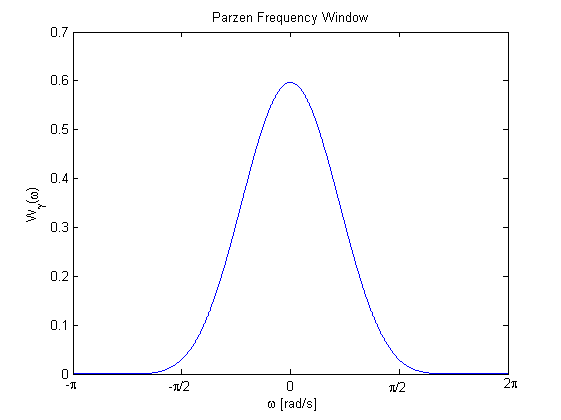
\includegraphics[width=0.7\textwidth]{pics/parzen}
\caption{}
\label{pic:}
\end{figure}



Here $\gamma$ is the parameter of smoothness. For $\gamma \rightarrow \infty$ the window $W_\gamma(\omega)$ has no effect. For $\gamma \rightarrow 0^+$ the smoothing becomes more prominent. The smoothing of the transfer function is generally a biased method which tries to minimize its variance. Depending on the smoothing parameter $\gamma$, one could obtain a function with a high bias, but low variance (high smoothing), or low bias with a higher variance (low smoothing). \\

Figure \ref{} displays the Bode plot of the non-smoothed transfer function estimate compared with smoothed estimates using different values of $\gamma$.


\begin{figure}[H]
\centering
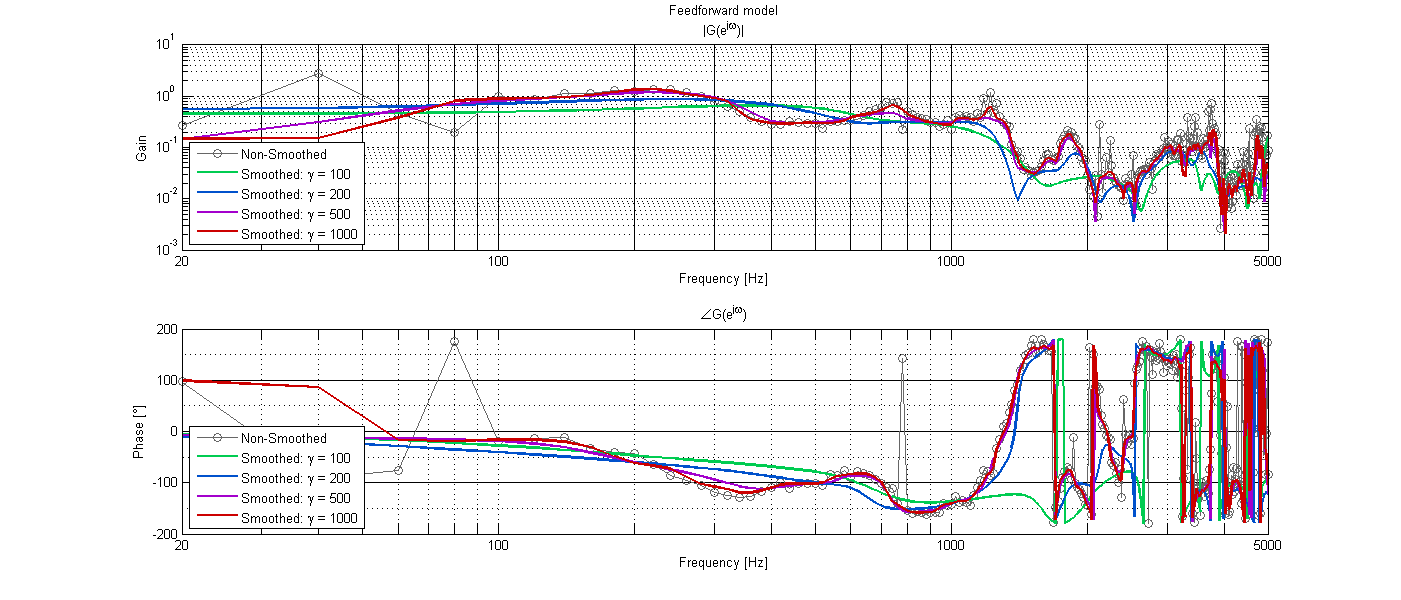
\includegraphics[width=1.0\textwidth]{pics/FF_Smoothing}
\caption{}
\label{pic:}
\end{figure}



\subsection{Subspace Identification}

Although linear systems are usually described in the frequency domain, state-space models can be used as a natural way of representing multi-variable parametric systems. Therefore, most implementations of control theory tools use state-space representations. There is a great number of algorithms that can be applied when time-domain measurements are available. Among the non-iterative algorithms we find the N4SID algorithm, a subspace identification algorithm that generates discrete state-space models without having to perform an explicit parameterization of the model set. The algorithm estimates subspace-based models, where the transfer function is rather insensitive to small changes in the matrix elements. This presents us with the possibility of identifying high order systems. \\

The method I used for the next part of the analysis uses the frequency domain identification algorithm proposed by \ref{}, which uses samples of the transfer function and delivers a minimal state-space model. Singular value decomposition (SVD) of a noisy data matrix has to be performed a priori in order to optimize the system order and only then can the algorithm be performed. The main advantages are the possibility of using a non-uniform frequency grid for the input frequency-domain data and its consistency (unbiased) over noise and correctness. 


\subsubsection{Order analysis}

As mentioned above, the order of the system has to be known a priori in order to use the N4SID algorithm. The following calculations are done. The noisy data matrix $\textbf{G}$ as well as the complex matrix $\textbf{W}_\text{m}$ are defined:
\[
\textbf{G} = \frac{1}{\sqrt{M}}
\begin{bmatrix}
G_1 & G_2 & \dots & G_M \\
e^{j\omega_1}G_1 & e^{j\omega_2}G_2 & \dots & e^{j\omega_M}G_M \\
e^{j2\omega_1}G_1 & e^{j2\omega_2}G_2 & \dots & e^{j2\omega_M}G_M \\
\vdots & \vdots & \ddots & \vdots \\
e^{j(q-1)\omega_1}G_1 &e^{j(q-1)\omega_2} G_2 & \dots & e^{j(q-1)\omega_M}G_M 
\end{bmatrix} \]
and

\[
\textbf{W}_m = \frac{1}{\sqrt{M}}
\begin{bmatrix}
1 & 1 & \dots & 1 \\
e^{j\omega_1} & e^{j\omega_2} & \dots & e^{j\omega_M} \\
e^{j2\omega_1} & e^{j2\omega_2} & \dots & e^{j2\omega_M} \\
\vdots & \vdots & \ddots & \vdots \\
e^{j(q-1)\omega_1} &e^{j(q-1)\omega_2} & \dots & e^{j(q-1)\omega_M} 
\end{bmatrix}\]

After this, a QR decomposition can be done in the following way:

\[\begin{bmatrix}
\Re(\textbf{W}_m) & \Im(\textbf{W}_m) \\
\Re(\textbf{G}) & \Im(\textbf{G})
\end{bmatrix} = 
\begin{bmatrix}
\textbf{R}_{11} & 0 \\
\textbf{R}_{21} & \textbf{R}_{22}
\end{bmatrix}\cdot
 \begin{bmatrix}
\textbf{Q}_1^T  \\
\textbf{Q}_2^T
\end{bmatrix}
\]
And a cholesky decomposition in the following way:
\[\textbf{K}\textbf{K}^T = \alpha\;\Re(\textbf{W}_p\,\text{diag}(R_1,R_2,\dots, R_M)\textbf{W}_p^*)\]

Where $()^*$ represents the conjugate transpose operator. Finally we calculate the SVD in the following way:

\[\textbf{K}^{-1}\textbf{R}_{22} = U\Sigma V^T\]

Since we are only interested in seeing the relations between the singular values, the $\alpha$ parameter in the cholesky decomposition has no interest. The values of $R_1, R_2, \dots$ correspond to the covariances of the noise, known a priori. Since we assumed that we're dealing with white noise, the covariance matrix is some multiple of the identity matrix. In this context are $\omega_1, \omega_2,\dots,\omega_M$ the sampled frequencies of our transfer function. It is not a uniform grid, because we only have information until 5 kHz, which is below the nyquist frequency (22.05 kHz). The parameters $q$ and $p$ have to be chosen a priori and only have have to be larger than the order of the real system (without noise)\\

What we expect to see, is a discrepancy between singular values. This way it should be easy to see how many belong to real states (order of the system) and which ones are "noise-states".

\subsubsection{N4SID Algorithm}

As mentioned above. The N4SID Algorithm takes as input the order of the system, calculated with the SVD analysis, and the noisy transfer function samples calculated above. 

\subsubsection{Optimal Parameters}

Unfortunately, the order analysis did not deliver any satisfactory results. Since there is no clear discrepancy between singular values. The real order of the system is therefore not clear. In the Appendix \ref{} one can see the signular value analysis for little, middle and a lot of smoothing for both setups. Since an order analysis was not possible to do, I took the approach of optimizing the parameters $\gamma$ and $n$ such that the rooth-mean-square error (RMS) is minimized when validating with the sweep signal responses. In other words, I generated an estimated output signal running the measured sweep sine input signal (in the headphone and chin microphone, for the FB and FF respectively) through the identified model. The root-mean-square error of the difference of the estimated and real output is calculated for each pair of $\gamma$ and $n$ in the following way:

\[\hat{\gamma} \quad\text{s.t.}\quad RMS(\hat{\gamma}) = \min\limits_\gamma RMS(\gamma)\]

where:

\[RMS(\gamma) = \frac{1}{N_1 + N_2} \sqrt{\sum\limits_{i=1}^{N_1}(y_1(k)-y_{\text{est},1}(k))+\sum\limits_{i=1}^{N_2}(y_2(k)-y_{\text{est},2}(k))}\]

Here are $y_1(k)$ and $y_2(k)$ the real outputs (ear channel in each, the FB and the FF setup) to both sweep sign responses that were acquired per setup. On the other hand, $y_{\text{est},1}(k)$ and $y_{\text{est},2}(k)$ are the estimated outputs.\\

A very important feature we want to keep in the estimated model is stability. We want a model that is stable, and this we have to search for the optimal parameters that also fulfil this requisit.\\

To analyse the RMS I searched over all models of order $n=1$ to $n = 20$ coming from a smoothed estimate of $\gamma = 10$ until $\gamma = 1000$ in steps of 10. Since those models are going to be use for control purposes, we want to keep the order as low as possible, therefore we don't search for orders higher than 20. For the smoothing parameter I set the searching limit at $\gamma = 1000$. As we see in Figures \ref{} and \ref{} smoothing parameters higher than 1000 overfit the noisy response, which adds unnucessary information. \\



\section{Results and Discussion}

\subsection{Feedback Model}
The optimization problem delivered the following result for the FB model (Figure \ref{}):

\begin{table}[H]
\centering
    \begin{tabular}{c|c|c}
    
    $\gamma$ & $n_\text{order}$ & RMS \\ \hline
    500      & 7                &  4.9381E-6   \\ 
    \end{tabular}
\end{table}

In Figure \ref{} we see the bode plot of the FB estimated system compared to the smoothed and noisy estimates. We see that until 3000 Hz the final estimation follows the trend of the noisy response in amplitude an phase rather accurately. After that, the trend is followed with less accuracy by the estimated model. Towards 5 kHz there is a roll-off in the estimation that is not to be seen by the trend of the noisy estimate. It is rather hard to interpret the physical modification of the signal that this transfer function represents, since the input is the measured voltage applied to a headphone (not the actual measurement of the sound it produces) and the output the sound inside the helmet. The fact that most of the transfer function has a gain higher than 1, doesn't mean, therefore, that the sound gets amplified (We would actually expect the opposite).  \\


\begin{figure}[H]
\centering
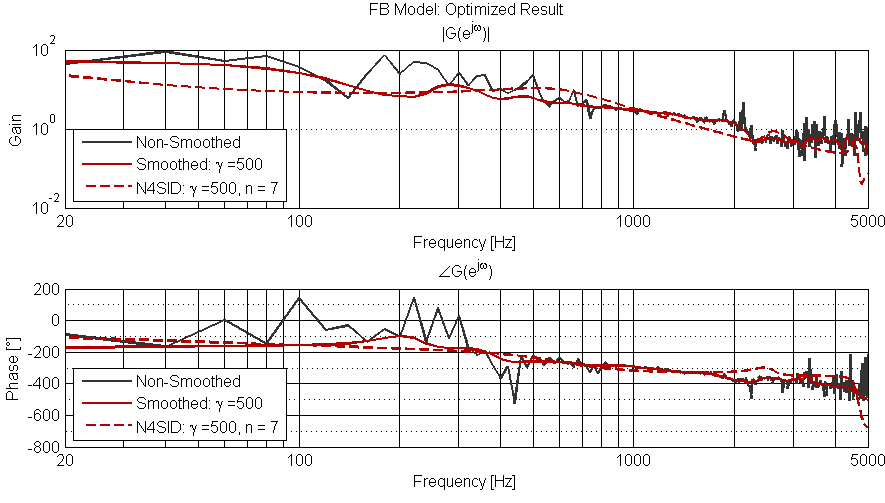
\includegraphics[width=1.0\textwidth]{pics/results_FB}
\caption{}
\label{pic:}
\end{figure}

In the following plot (Figure \ref{}) we see that the system is stable, since all of its poles are inside the unit circle of the Gauss-plane. As mentioned before, it is plausible to have assumed this a priori, since every frequency would eventually get damped to death inside of the helmet, even if there might be complex sound effects like ressonances and echoes. One of the poles is, however, much nearer to the unit circle axis. This leads to a slower roll-off of the impulse response, compared to the FF model that will be shown further down. We also observe non minimum phase zeros which bring the system to "lie" (start in a certain direction and then changeit) in the impulse response (Figure \ref{}).

\begin{figure}[H]
\centering
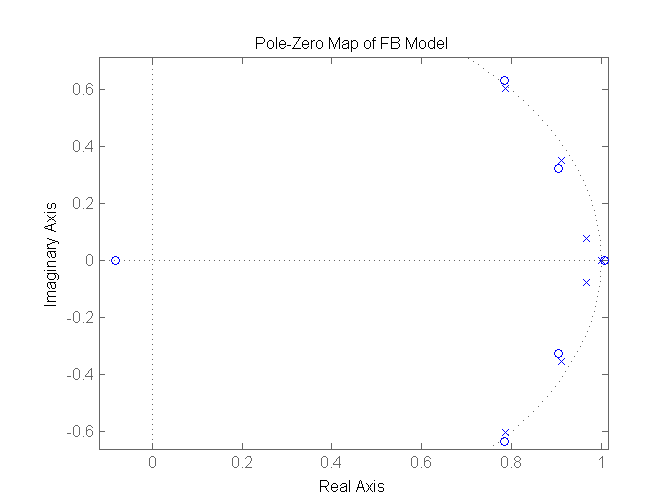
\includegraphics[width=1.0\textwidth]{pics/pole_FB}
\caption{}
\label{pic:}
\end{figure}

Initially, I didn't take in account the first 3 seconds of the filtered noise response (since the noise starts) to avoid including the transient part in the system identification process.  Figure \ref{} shows that the impulse response of the estimated model indeed decreases sufficiently fast within the first 3 seconds to assume that the transient of the noise response is gone in the data that was taken for the identification.

\begin{figure}[H]
\centering
\begin{subfigure}[b]{0.5\textwidth}
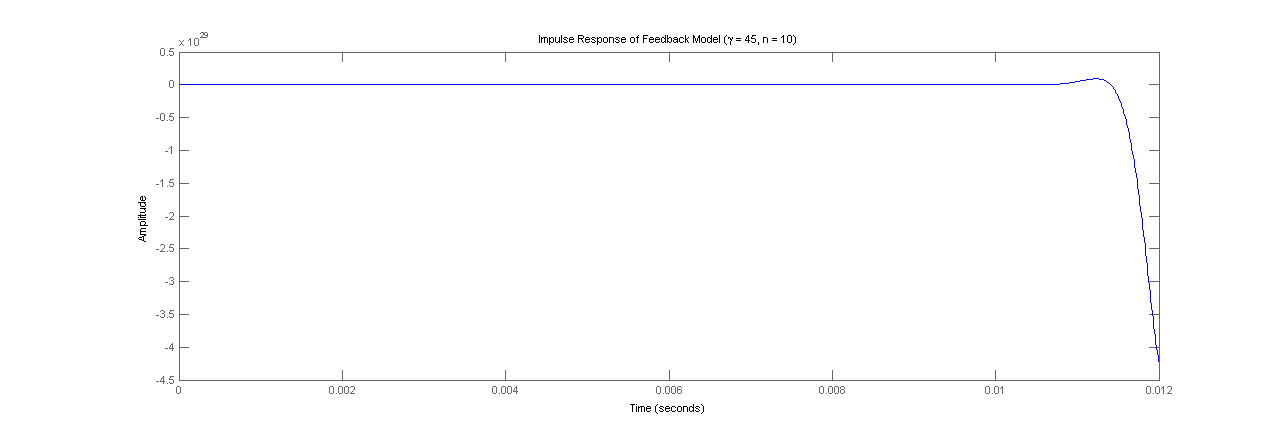
\includegraphics[width=1.0\textwidth]{pics/impulse_FB}
\caption{}
\label{pic:}
\end{subfigure}\;\begin{subfigure}[b]{0.5\textwidth}
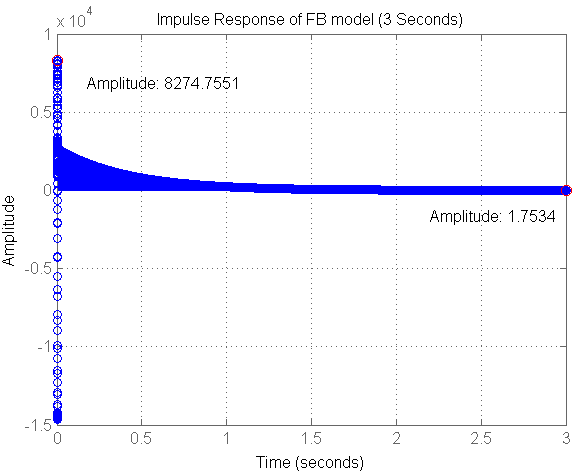
\includegraphics[width=1.0\textwidth]{pics/impulse_FB_3sec}
\caption{}
\label{pic:}
\end{subfigure}

\end{figure}

\subsection{Feedforward Model}
For the feedforward model identifcation we received the following result from our optimization problem. 

\begin{table}[H]
\centering
    \begin{tabular}{c|c|c}
    
    $\gamma$ & $n_\text{order}$ & RMS \\ \hline
    90      & 5                &  3.6571E-05   \\ 
    \end{tabular}
\end{table}

Figure \ref{} shows the bode plot of the estimated model compared to the smoothed and noisy models. The estimation here shows a better fit in amplitude, but a more chaotic behaviour in the phase plot. Due to the agressive behaviour of the phase plots, an unwrapping of the phase was not possible like it was done for the feedback model. The RMS in this case is almost one order greater than in the feedback model, which is clear on the phase plot. Fortunately, the estimated model follows the trend of the noisy and smoothed models much better in the bode plot than in the case of the feedback model. The result is therefore satisfactory in lower and higher frequencies.\\

\begin{figure}[H]
\centering
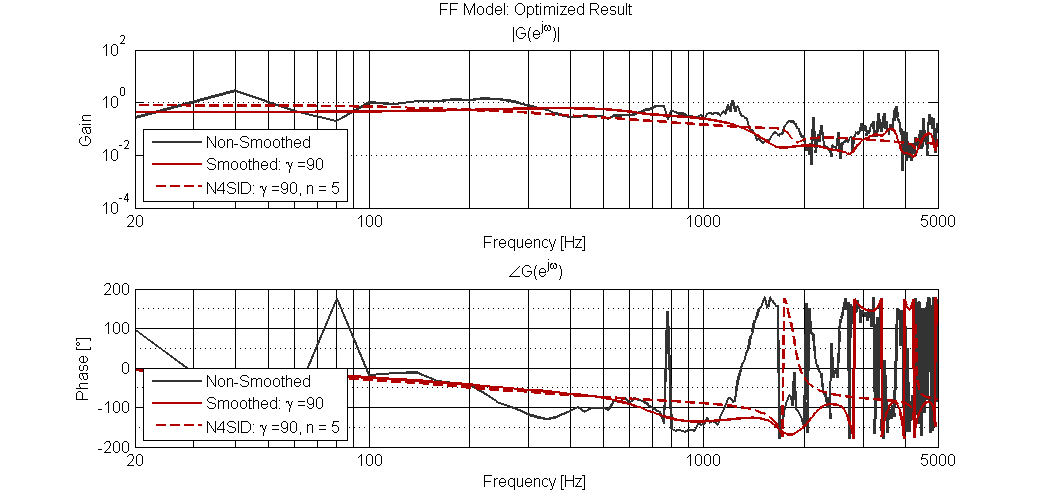
\includegraphics[width=1.0\textwidth]{pics/results_FF}
\caption{}
\label{pic:}
\end{figure}

The bode plot shows always an amplitude lower than 1. This is what one would expect intuitically from the experiment, since the input signal comes from a source that closer to the sound source (chin channel) than the output (ear channel). Contrary to the feedback case, here are both, input and output signals voltage measurements of sound pressure.

\begin{figure}[H]
\centering
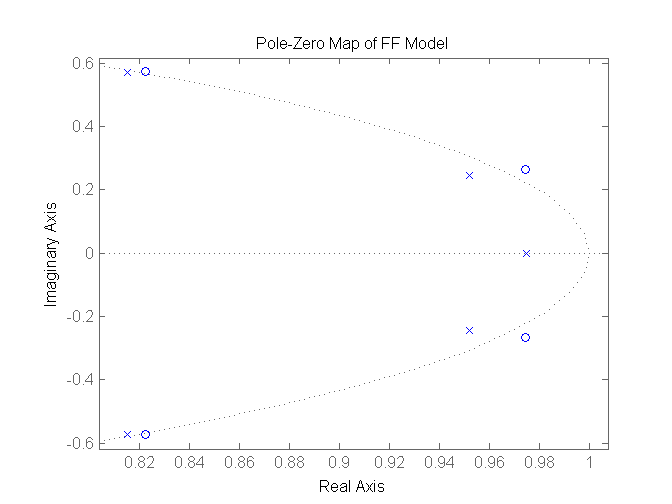
\includegraphics[width=1.0\textwidth]{pics/pole_FF}
\caption{}
\label{pic:}
\end{figure}

Like in the FB case, we see in Figure \ref{} that the system has all poles inside the unit circle. This time there are only minimalphase zeros. We observe the stability provided by the poles as well as no system "lying" in the impulse response in Figure \ref{}. 

\begin{figure}[H]
\centering
\begin{subfigure}[b]{0.5\textwidth}
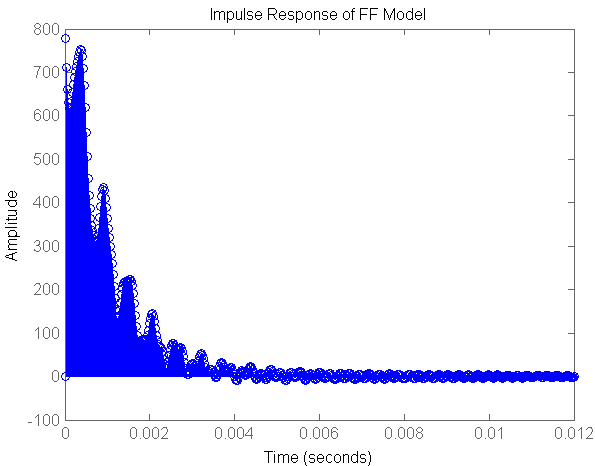
\includegraphics[width=1.0\textwidth]{pics/impulse_FF}
\caption{}
\label{pic:}
\end{subfigure}\;\begin{subfigure}[b]{0.5\textwidth}
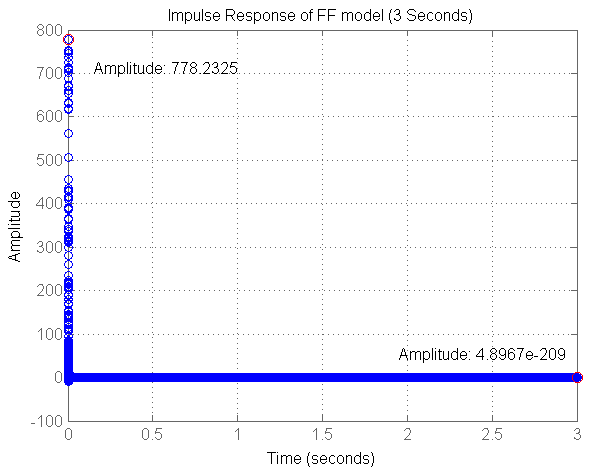
\includegraphics[width=1.0\textwidth]{pics/impulse_FF_3sec}
\caption{}
\label{pic:}
\end{subfigure}

\end{figure}

Figure \ref{} shows furthermore that our assumption that the transient effect wears off within 3 seconds is plausible, since the amplitude decay decreases drastically in that time.

For detailed numerical information about the identified systems i.e. transfer functions, system matrices, poles and zeros, please refere to the Appendix.

\section{Conclusion}

As mentioned before, the results in both cases were very satisfactory in terms of following the trend of the noisy estimate in the critical frequency range for noise (accoridng to \ref{}) while preserving stability properties and low order. Since no further specifications were given that could give a better control performance, I find the optimization approach that minimizes the RMS good enough.\\

The models lack of accuracy in the higher frequencies used for identification. If one was to use the methods used here, i.e. smoothing and n4sid subspace identification and wished for higher accuracy, stability couldn't be preserved (better unstable fits were actually found).\\

Here we dealt with a model that works with discrete inputs and outputs, if one was interested in the actual acoustic model that modifies the sound waves one could use bilinear transformation to create a continuous model. The relations between sound pressure level at the microphone location and the amplitude of the signal it produces should be known to be able to do this.

